% ===========================================================================
% MODELO DE RELATORIO  ·  ENE0046 Laboratorio de Eletronica  ·  2026/2
%
% Como usar
%   1. Preencha o bloco IDENTIFICACAO logo abaixo.
%   2. Deixe comentados os autores que nao existirem. Um autor fica centralizado,
%      dois dividem a linha, tres ocupam tercos.
%   3. Substitua o texto de cada secao pelo seu. As orientacoes que estao la
%      dizem o que se espera em cada uma.
%   4. Compile com pdflatex duas vezes, ou com latexmk -pdf.
%
% Estrutura
%   Roteiro 1 nao tem bancada: use so a subsecao 4.1 e a 5.1, e compare o calculo
%   analitico com a simulacao de projeto.
%   Roteiros 2 a 7 usam a estrutura inteira.
%
% O arquivo estilo-relatorio.tex deve estar na mesma pasta deste arquivo. A logo
% e as figuras ficam organizadas na subpasta imgs/, como no relatorio preenchido.
% ===========================================================================
\documentclass[11pt,a4paper]{article}
% !TeX root = modelo-relatorio.tex
% Formatacao do relatorio. Compile o modelo-relatorio.tex, nao este arquivo.
\usepackage[T1]{fontenc}
\usepackage[utf8]{inputenc}
\usepackage[brazil]{babel}
\usepackage[a4paper,top=1.6cm,bottom=1.8cm,left=2.1cm,right=2.1cm]{geometry}
\usepackage[default]{lato}
\usepackage{amsmath,amssymb}
\usepackage{siunitx}
\usepackage{graphicx}
\usepackage{booktabs,array,longtable,colortbl}
\usepackage{enumitem}
\usepackage{tcolorbox}
\usepackage{xcolor}
\usepackage{float}
\usepackage{tikz}
\usepackage{titlesec}
\usepackage{fancyhdr}
\usepackage{caption}
\usepackage{etoolbox}
\usepackage[colorlinks=true,linkcolor=azul,urlcolor=azul,citecolor=azul]{hyperref}
\tcbuselibrary{skins,breakable}

\definecolor{azul}{HTML}{0A4B8C}
\definecolor{azulclaro}{HTML}{E8F0F8}
\definecolor{verde}{HTML}{0B7A4B}
\definecolor{cinza}{HTML}{5B6672}
\definecolor{cinzaclaro}{HTML}{F4F6F8}
\definecolor{vinho}{HTML}{B04A4A}
\definecolor{vinhoclaro}{HTML}{FBF2F2}

\sisetup{output-decimal-marker={,}, per-mode=symbol}
\setlength{\parindent}{0pt}
\setlength{\parskip}{6pt plus 1pt}
\setlist{itemsep=3pt, topsep=4pt, parsep=0pt, leftmargin=1.3em}
\renewcommand{\arraystretch}{1.25}
\linespread{1.06}

% ---- secoes numeradas com marcador colorido -------------------------------
\titleformat{\section}[hang]
  {\Large\bfseries\color{azul}}
  {\raisebox{-1pt}{\tikz\node[fill=azul,text=white,rounded corners=2pt,
     inner sep=3pt,minimum width=20pt,align=center]{\bfseries\thesection};}}
  {10pt}{}
\titlespacing*{\section}{0pt}{16pt plus 3pt}{6pt}
\titleformat{\subsection}{\large\bfseries\color{cinza}}{\thesubsection}{8pt}{}
\titlespacing*{\subsection}{0pt}{11pt plus 2pt}{3pt}

% ---- legendas -------------------------------------------------------------
\captionsetup{font=small,labelfont={bf,color=azul},labelsep=period,skip=6pt}

% ---- identificacao --------------------------------------------------------
\newcommand{\autorA}{}\newcommand{\matA}{}
\newcommand{\autorB}{}\newcommand{\matB}{}
\newcommand{\autorC}{}\newcommand{\matC}{}
\newcommand{\autorum}[2]{\renewcommand{\autorA}{#1}\renewcommand{\matA}{#2}}
\newcommand{\autordois}[2]{\renewcommand{\autorB}{#1}\renewcommand{\matB}{#2}}
\newcommand{\autortres}[2]{\renewcommand{\autorC}{#1}\renewcommand{\matC}{#2}}

\newcommand{\disciplina}{ENE0046 · Laboratório de Eletrônica}
\newcommand{\semestre}{2026/2}
\newcommand{\turma}{}
\newcommand{\roteironum}{}
\newcommand{\roteirotema}{}
\newcommand{\aturma}[1]{\renewcommand{\turma}{#1}}
\newcommand{\roteiro}[2]{\renewcommand{\roteironum}{#1}\renewcommand{\roteirotema}{#2}}

\newcommand{\umautor}[2]{%
  \begin{minipage}[t]{\dimexpr\linewidth-4pt\relax}\centering
    \parbox[t][30pt][t]{\linewidth}{\centering
      {\fontsize{10.5}{12.5}\selectfont #1}}\\[-2pt]
    {\color{cinza}\fontsize{9}{11}\selectfont\texttt{#2}}
  \end{minipage}}

\newcounter{nautores}
\newcommand{\blocoautores}{%
  \setcounter{nautores}{0}%
  \ifdefempty{\autorA}{}{\stepcounter{nautores}}%
  \ifdefempty{\autorB}{}{\stepcounter{nautores}}%
  \ifdefempty{\autorC}{}{\stepcounter{nautores}}%
  \ifnum\value{nautores}=0
    \begin{center}\color{vinho}\bfseries
      Preencha ao menos um autor no preâmbulo do arquivo.
    \end{center}
  \else
    \begin{center}
    \ifcase\value{nautores}\or
      % --- um autor: ocupa o centro
      \begin{minipage}{0.5\textwidth}\umautor{\autorA}{\matA}\end{minipage}%
    \or
      % --- dois autores: metades
      \begin{minipage}{0.42\textwidth}\umautor{\autorA}{\matA}\end{minipage}\hspace{0.04\textwidth}%
      \begin{minipage}{0.42\textwidth}\umautor{\autorB}{\matB}\end{minipage}%
    \or
      % --- tres autores: tercos
      \begin{minipage}{0.31\textwidth}\umautor{\autorA}{\matA}\end{minipage}\hspace{0.015\textwidth}%
      \begin{minipage}{0.31\textwidth}\umautor{\autorB}{\matB}\end{minipage}\hspace{0.015\textwidth}%
      \begin{minipage}{0.31\textwidth}\umautor{\autorC}{\matC}\end{minipage}%
    \fi
    \end{center}
  \fi}

% ---- cabecalho do relatorio -----------------------------------------------
\newcommand{\capa}{%
\begin{tcolorbox}[colback=azul,colframe=azul,boxrule=0pt,arc=4pt,
  left=16pt,right=16pt,top=13pt,bottom=13pt]
\color{white}
\begin{minipage}{0.76\textwidth}
  {\fontsize{9}{11}\selectfont\textbf{\MakeUppercase{\disciplina{} · \semestre{}}}}\\[6pt]
  {\fontsize{22}{25}\selectfont\bfseries Relatório do Roteiro \roteironum}\\[3pt]
  {\fontsize{12.5}{15}\selectfont \roteirotema}
\end{minipage}\hfill
\begin{minipage}{0.2\textwidth}\raggedleft
  \colorbox{white}{\hspace{2pt}\raisebox{-2pt}{
\includegraphics[height=30pt]{imgs/logo-unb.png}}\hspace{2pt}}
\end{minipage}
\end{tcolorbox}
\vspace{10pt}
\blocoautores
\ifdefempty{\turma}{}{%
  \begin{center}{\color{cinza}\fontsize{9}{11}\selectfont Turma \turma}\end{center}}
\vspace{4pt}
{\color{azulclaro}\hrule height 2pt}
\vspace{2pt}}

% ---- caixas auxiliares ----------------------------------------------------
\newtcolorbox{formula}{colback=azulclaro,colframe=azul,boxrule=0.8pt,arc=3pt,
  left=12pt,right=12pt,top=9pt,bottom=9pt}
\newtcolorbox{nota}[1]{colback=cinzaclaro,colframe=cinza,boxrule=0.8pt,arc=3pt,
  left=10pt,right=10pt,top=7pt,bottom=7pt,
  title={\textbf{#1}},fonttitle=\small\bfseries,coltitle=white,colbacktitle=cinza}
\newenvironment{resumo}
  {\vspace{6pt}\begin{center}\begin{minipage}{0.92\textwidth}
   \begin{tcolorbox}[colback=cinzaclaro,colframe=cinzaclaro,boxrule=0pt,arc=3pt,
     left=14pt,right=14pt,top=10pt,bottom=10pt,
     borderline west={2.5pt}{0pt}{azul}]
   {\color{azul}\fontsize{8}{10}\selectfont\textbf{RESUMO}}\\[4pt]
   \small}
  {\end{tcolorbox}\end{minipage}\end{center}\vspace{2pt}}

\newtcolorbox{espec}{colback=azulclaro,colframe=azul,boxrule=0.8pt,arc=3pt,
  left=12pt,right=12pt,top=9pt,bottom=9pt,
  title={\textbf{Especificação da matrícula}},fonttitle=\bfseries,
  coltitle=white,colbacktitle=azul}

\newtcolorbox{especbancada}{colback=azulclaro,colframe=azul,boxrule=0.8pt,arc=3pt,
  left=12pt,right=12pt,top=9pt,bottom=9pt,
  title={\textbf{Especificação da Equipe}},fonttitle=\bfseries,
  coltitle=white,colbacktitle=azul}

% ---- rodape ---------------------------------------------------------------
\pagestyle{fancy}\fancyhf{}
\renewcommand{\headrulewidth}{0pt}
\renewcommand{\footrulewidth}{0.4pt}
\fancyfoot[L]{\color{cinza}\fontsize{8}{10}\selectfont \disciplina{} · \semestre{} · Roteiro \roteironum}
\fancyfoot[R]{\color{cinza}\fontsize{8}{10}\selectfont \thepage}

\newlist{referencias}{itemize}{1}
\setlist[referencias]{label={}, leftmargin=1.1em, itemindent=-1.1em,
                     itemsep=3pt, topsep=2pt, parsep=0pt}

\newcommand{\mat}[1]{\texttt{\textbf{#1}}}


% --------------------------- IDENTIFICACAO ---------------------------------
\roteiro{1}{Simulação de Circuitos: Introdução ao LTspice}
\aturma{03}

\autorum{Lurian Correia Lima}{22/2005395} 
\autordois{Guilherme Cardoso Oliveira da Silva Júnior}{23/1038626}
\autortres{Daniel Campos Silva}{23/1036775}
% ---------------------------------------------------------------------------

\begin{document}
\capa

\begin{resumo}
% Escreva este parágrafo por último, com 100 a 150 palavras. Diga o que você projetou, sob
% qual especificação, o que simulou ou mediu, o principal resultado numérico e a que
% conclusão chegou. Quem ler só este parágrafo deve saber o que você fez e o que encontrou.
\end{resumo}

\section{Introdução}

% Comece pelo problema, e não pelo circuito. Que necessidade de engenharia deu origem a esta
% topologia, onde você a encontraria em um equipamento real e o que aconteceria sem ela. Duas
% ou três referências ajudam aqui.

% Depois estreite o foco: que aspecto você vai investigar, sob quais condições, e por que
% vale a pena verificá-lo. Se o roteiro impõe alguma restrição de projeto que parece
% arbitrária, aproveite para explicar a razão dela.

% No último parágrafo, diga qual é o objetivo deste relatório e como o texto está
% organizado, seção a seção.

\section{Fundamentação teórica}

% Deduza as expressões que você vai usar mais adiante, partindo das leis de circuito.
% Numere as equações que forem retomadas no restante do texto.

% \begin{equation}
% H(j\omega) = \frac{1}{1+j\omega RC}
% \label{eq:exemplo}
% \end{equation}

% Toda grandeza que aparecer nos resultados precisa ter sido apresentada aqui. Explique o que
% cada termo significa fisicamente, não apenas o que a letra representa. Registre as hipóteses
% que você está assumindo, como linearidade ou idealidade dos componentes: se alguma delas
% não se sustentar no experimento, você vai retomá-la na discussão.

% Se o circuito tiver regimes de funcionamento distintos, apresente cada um e diga o que os
% separa.

\section{Especificação e projeto}

\begin{espec}

\textbf{Matrícula \mat{23/1038626}.} Considerando os nove dígitos na forma ABCDEFGHI:

\begin{equation}
    A=2,\; B=3,\; C=1,\; D=0,\; E=3,\; F=8,\; G=6,\; H=2,\; I=6
\end{equation}

A partir desses valores, as especificações individuais exigidas pelo roteiro são:

\begin{itemize}
    \item \textbf{Comparador:} \hfill\break
    $R_1 = I\text{ k}\Omega = 6\text{ k}\Omega$ e $R_2 = AB\text{ k}\Omega = 23\text{ k}\Omega$.

\vspace{0.3cm}

    \item \textbf{Integrador:} \hfill\break
    $R_3 = 33\text{ k}\Omega$ e $C_1 = 1\text{ }\mu\text{F}$.
    
    \vspace{0.3cm}
    
    \item \textbf{Conformador:} \hfill\break
    Entrada com a amplitude da onda quadrada, senoide de amplitude $A = (0{,}45 + H/40) V_{\text{T}}$ e quebras em $\theta_{1} = 30^\circ$, $\theta_2 = 50^\circ$ e $\theta_3 = 75^\circ$. (Para $H=2$, a amplitude projetada é $A = 0{,}50 V_{\text{T}}$).
\end{itemize}

\end{espec}

Os componentes da série comercial E12 selecionados para atender a cada especificação, bem como o desenvolvimento analítico para o seu dimensionamento, são detalhados a seguir:

\begin{itemize}

    \item \textbf{Comparador com Histerese ($R_1$ e $R_2$):} \hfill\break
    A especificação determina $R_1 = 6\,\mathrm{k}\Omega$ e $R_2 = 23\,\mathrm{k}\Omega$. Como o roteiro permite a utilização de dois resistores em série para compor os valores exatos, adotou-se para a série E12: $R_1 = 3{,}3\,\mathrm{k}\Omega + 2{,}7\,\mathrm{k}\Omega = 6\,\mathrm{k}\Omega$ e $R_2 = 22\,\mathrm{k}\Omega + 1\,\mathrm{k}\Omega = 23\,\mathrm{k}\Omega$. O dimensionamento atende integralmente ao valor teórico sem desvios, resultando na amplitude teórica para a onda triangular de $V_{tri} = \frac{R_1}{R_2}V_{sat} = \frac{6}{23}V_{sat} \approx 0{,}261 V_{sat}$ (Eq. 2).

    \item \textbf{Gerador de Ondas (Integrador e Amplificador):} \hfill\break
    O filtro integrador utiliza de forma direta os componentes padrões $R_3 = 33\,\mathrm{k}\Omega$ e $C_1 = 1\,\mu\mathrm{F}$. Inserindo os resistores exatos do comparador na Equação 3, a frequência de oscilação teórica estabelece-se em:
    \[ f = \frac{R_2}{4 R_1 R_3 C_1} = \frac{23\text{ k}}{4 \times 6\text{ k} \times 33\text{ k} \times 1\mu} \approx 29{,}04\text{ Hz} \]
    Para o estágio do amplificador não inversor do conformador, a fim de recuperar a amplitude da onda quadrada, o ganho teórico deve ser $G = \frac{R_2}{R_1} = \frac{23}{6} \approx 3{,}833$. Sendo a topologia não inversora dada por $G = 1 + \frac{R_f}{R_g}$, a razão necessária é $\frac{R_f}{R_g} = \frac{17}{6} \approx 2{,}833$. Utilizando resistores da série E12, definiu-se $R_g = 12\,\mathrm{k}\Omega$ e $R_f = 33\,\mathrm{k}\Omega + 1\,\mathrm{k}\Omega = 34\,\mathrm{k}\Omega$. Com isso, o ganho real é $1 + \frac{34}{12} = \frac{46}{12} = 3{,}833$, zerando completamente o desvio em relação ao ganho teórico pretendido.

    \item \textbf{Divisor e Conformador a Diodos ($R_4$ a $R_7$ e Malhas de Inclinação):} \hfill\break
    Projetando o circuito para uma tensão de saturação típica $V_T = V_{sat} \approx 14\text{ V}$ (alimentação $\pm15\text{ V}$), a amplitude da senoide a ser aproximada é:
    \[ A = \left(0{,}45 + \frac{2}{40}\right)14 = 0{,}50 \times 14 = 7\text{ V} \]
    Os limiares teóricos de condução (Eq. 5), correspondentes aos ângulos de quebra, são calculados por $V_k = A \text{ sen}(\theta_k)$:
    \begin{align*}
        V_1 &= 7 \text{ sen}(30^\circ) = 3{,}500\text{ V} \\
        V_2 &= 7 \text{ sen}(50^\circ) \approx 5{,}362\text{ V} \\
        V_3 &= 7 \text{ sen}(75^\circ) \approx 6{,}761\text{ V}
    \end{align*}
    
    Dimensionamento do divisor (Eq. 6): Arbitrando $R_T = 22\,\mathrm{k}\Omega$ (valor dentro da faixa de 15 a 30 $\mathrm{k}\Omega$), calculam-se os resistores para $V_{CC} = 15\text{ V}$:
    \begin{align*}
        R_7 &= R_T \frac{V_1 - 0{,}7}{V_{CC}} = 22\text{k} \frac{3{,}5 - 0{,}7}{15} \approx 4{,}106\,\mathrm{k}\Omega \\
        R_6 &= R_T \frac{V_2 - 0{,}7}{V_{CC}} - R_7 = 22\text{k} \frac{5{,}362 - 0{,}7}{15} - 4{,}106\text{k} \approx 2{,}731\,\mathrm{k}\Omega \\
        R_5 &= R_T \frac{V_3 - 0{,}7}{V_{CC}} - R_7 - R_6 = 22\text{k} \frac{6{,}761 - 0{,}7}{15} - 6{,}837\text{k} \approx 2{,}052\,\mathrm{k}\Omega \\
        R_4 &= R_T - R_5 - R_6 - R_7 = 22\text{k} - 8{,}889\text{k} \approx 13{,}111\,\mathrm{k}\Omega
    \end{align*}
    Mapeando para a série E12, adotaram-se as associações exatas fornecidas: $R_7 = 3{,}9\,\mathrm{k}\Omega + 150\,\Omega = 4{,}05\,\mathrm{k}\Omega$; $R_6 = 2{,}7\,\mathrm{k}\Omega$; $R_5 = 1{,}8\,\mathrm{k}\Omega + 220\,\Omega = 2{,}02\,\mathrm{k}\Omega$; e $R_4 = 12\,\mathrm{k}\Omega + 1{,}2\,\mathrm{k}\Omega = 13{,}2\,\mathrm{k}\Omega$. O somatório realiza um $R_{T,\text{real}} = 21{,}97\,\mathrm{k}\Omega$.

    Dimensionamento das malhas de inclinação (Eq. 7): O resistor de entrada isola o divisor, definido em $10\times$ o valor de $R_T$. Fixou-se $R_{in} = 220\,\mathrm{k}\Omega$. Os valores da onda triangular nos ângulos de quebra são dados por $V_\theta = V_T \frac{\theta}{90^\circ}$:
    \[ V_{\theta_2} = 14 \frac{50^\circ}{90^\circ} \approx 7{,}777\text{ V} \quad \text{e} \quad V_{\theta_3} = 14 \frac{75^\circ}{90^\circ} \approx 11{,}666\text{ V} \]
    Aplicando a equação para o primeiro diodo de inclinação (referenciado como $R_2$ no roteiro, e $R_{c2}$ aqui para evitar ambiguidade):
    \[ R_{c2} = R_{in} \left( \frac{V_{\theta_2} - V_1}{V_{\theta_2} - V_2} - 1 \right) = 220\text{k} \left( \frac{7{,}777 - 3{,}500}{7{,}777 - 5{,}362} - 1 \right) \approx 169{,}61\,\mathrm{k}\Omega \]
    Adotou-se a associação $R_{c2} = 150\,\mathrm{k}\Omega + 18\,\mathrm{k}\Omega = 168\,\mathrm{k}\Omega$.
    
    Para o segundo diodo ($R_{c3}$), calcula-se primeiro o nível intermediário ideal $V^*$:
    \[ V^* = V_{\theta_3} - \frac{R_{in}(V_{\theta_3} - V_1)}{R_{in} + R_{c2}} = 11{,}666 - \frac{220\text{k}(11{,}666 - 3{,}500)}{220\text{k} + 168\text{k}} \approx 7{,}036\text{ V} \]
    Por fim, a resistência teórica do último segmento é:
    \[ R_{c3} = R_{in} \left( \frac{V^* - V_2}{V^* - V_3} - 1 \right) = 220\text{k} \left( \frac{7{,}036 - 5{,}362}{7{,}036 - 6{,}761} - 1 \right) \approx 1{,}120\,\mathrm{M}\Omega \]
    Na série E12, adotou-se a associação $R_{c3} = 1\,\mathrm{M}\Omega + 47\,\mathrm{k}\Omega = 1{,}047\,\mathrm{M}\Omega$.

\end{itemize}

A tabela abaixo resume os parâmetros teóricos de projeto e os efetivamente adotados:

\begin{center}
\renewcommand{\arraystretch}{1.2}
\begin{tabular}{@{}lrrr@{}}
\toprule
\textbf{Grandeza} & \textbf{Teórico} & \textbf{Adotado (E12 associada)} & \textbf{Desvio} \\
\midrule
Resistor do Comparador ($R_1$) & $6{,}00\text{ k}\Omega$ & $6{,}00\text{ k}\Omega$ & $0{,}00\%$ \\
Resistor do Comparador ($R_2$) & $23{,}00\text{ k}\Omega$ & $23{,}00\text{ k}\Omega$ & $0{,}00\%$ \\
Frequência Astável ($f$) & $29{,}04\text{ Hz}$ & $29{,}04\text{ Hz}$ & $0{,}00\%$ \\
Ganho do Amplificador ($G$) & $3{,}833\text{ V/V}$ & $3{,}833\text{ V/V}$ & $0{,}00\%$ \\
Resistência de Entrada ($R_{in}$ Conformador) & $219{,}70\text{ k}\Omega$ & $220{,}00\text{ k}\Omega$ & $0{,}13\%$ \\
Resistência de Inclinação ($R_{c2}$ Conformador) & $169{,}61\text{ k}\Omega$ & $168{,}00\text{ k}\Omega$ & $-0{,}95\%$ \\
Resistência de Inclinação ($R_{c3}$ Conformador) & $1{,}120\text{ M}\Omega$ & $1{,}047\text{ M}\Omega$ & $-6{,}51\%$ \\
\bottomrule
\end{tabular}
\end{center}

% Transcreva os parâmetros que a sua matrícula determina, mostrando a conta a partir dos
% dígitos.

% \begin{espec}
% Matrícula \mat{00/0000000}. \\
% Preencha aqui os parâmetros calculados a partir dos dígitos, conforme o roteiro.
% \end{espec}

% Leve cada parâmetro até o valor de componente, deixando visível a expressão que você
% inverteu para chegar lá. Depois escolha o valor na série comercial e calcule o quanto essa
% escolha afasta você do valor ideal. A tabela abaixo organiza isso, e é ela que depois
% permite separar o que veio do projeto do que veio da montagem.

% \begin{center}
% \begin{tabular}{@{}lrrr@{}}
% \toprule
% \textbf{Grandeza} & \textbf{Teórico} & \textbf{Adotado} & \textbf{Desvio} \\
% \midrule
% & & & \\
% \bottomrule
% \end{tabular}
% \end{center}

% Se mais de uma combinação atender à especificação, diga por que escolheu esta, mostrando
% que as outras ficavam mais distantes.

\section{Metodologia}

% Conte o que você fez e com quais parâmetros, de modo que um colega consiga repetir sem
% precisar perguntar nada. Explique as escolhas que não são evidentes: por que essa faixa de
% varredura, por que esse passo de integração, por que esse intervalo de gravação.

% Inclua a figura do esquemático, com legenda que descreva o que ela mostra, e cite-a no
% texto, como na Figura~\ref{fig:exemplo}. Se uma figura não for mencionada em nenhum
% parágrafo, ela provavelmente não precisa estar aqui.

\subsection{Simulação de projeto, uma por integrante}

\subsubsection{Guilherme Cardoso Oliveira da Silva Júnior (23/1038626)}

\textbf{Configuração e Simulação dos Circuitos}

Para comprovar que o projeto atende às especificações apresentadas na Seção 3 (referentes ao comparador com histerese, integrador e conformador de onda), os três circuitos foram desenhados e simulados no LTspice, conforme a Figura~\ref{fig:circs_guilherme}. Em todas as análises, adotou-se a diretiva de regime transitório de 300 ms (\texttt{.tran 0 300m}). Os esquemáticos foram configurados da seguinte forma:

\begin{itemize}
    \item \textbf{Comparador com histerese (Fig.~\ref{fig:circs_guilherme}a):} O amplificador LM741 foi configurado com os resistores da malha de realimentação positiva $R_1$ e $R_2$ calculados a partir da matrícula ($6\text{ k}\Omega$ e $23\text{ k}\Omega$, implementados por associações em série). A entrada foi excitada por uma senoide de 10 Hz com amplitude de 10 V para provocar a comutação e revelar os limiares práticos de saturação e transição. 
    
    \item \textbf{Gerador de ondas (Fig.~\ref{fig:circs_guilherme}b):} Ao circuito anterior, adicionou-se um segundo estágio (integrador), que recebe a onda quadrada e a devolve em formato triangular. Esse integrador utiliza a especificação geral da turma de $R_3 = 33\text{ k}\Omega$ e $C_1 = 1\text{ }\mu\text{F}$. O pino não inversor de ambos os amplificadores operacionais foi devidamente aterrado, e o circuito partiu do repouso sem sinal de entrada externo (diretiva \texttt{startup}).

    \item \textbf{Cadeia completa e conformador a diodos (Fig.~\ref{fig:circs_guilherme}c):} Inseriu-se um terceiro estágio amplificador não inversor para igualar a amplitude do sinal triangular aos $\approx 14\text{ V}$ da onda quadrada (utilizando as associações para $R_f = 34\text{ k}\Omega$ e $R_g = 12\text{ k}\Omega$). Na saída, instalou-se o divisor resistivo e as malhas com seis diodos 1N4148. Para a avaliação do THD, a diretiva \texttt{.four 29.04 V(v\_sen)} foi introduzida no arquivo.
\end{itemize}

\begin{figure}[H]
\centering
\begin{minipage}{0.48\linewidth}
    \centering
    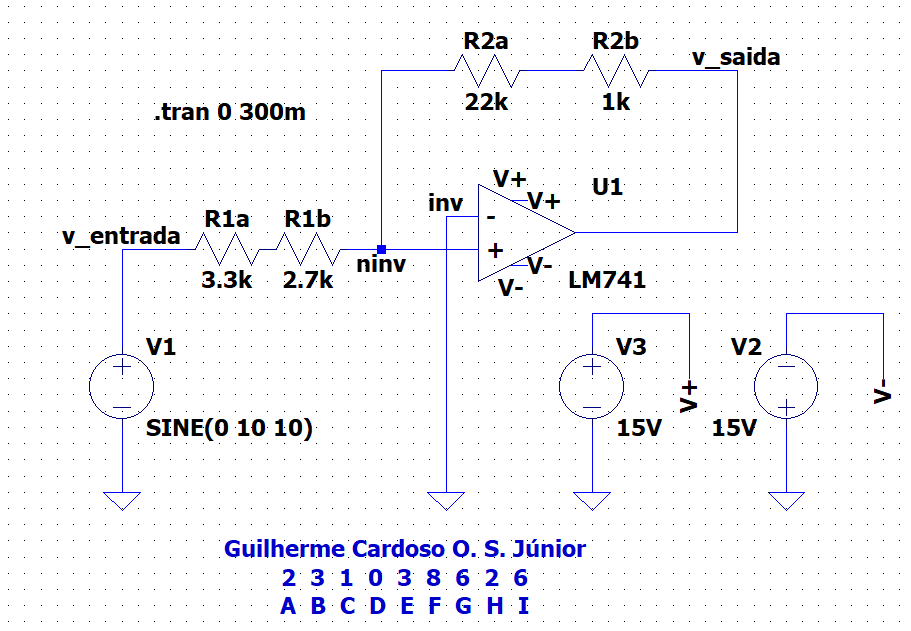
\includegraphics[width=\linewidth]{imgs/cardoso/esquematicos/item_1_esquematico.png}
    \vspace{2pt}
    {\small (a) Comparador com histerese excito por sinal senoidal externo.}
\end{minipage}\hfill
\begin{minipage}{0.48\linewidth}
    \centering
    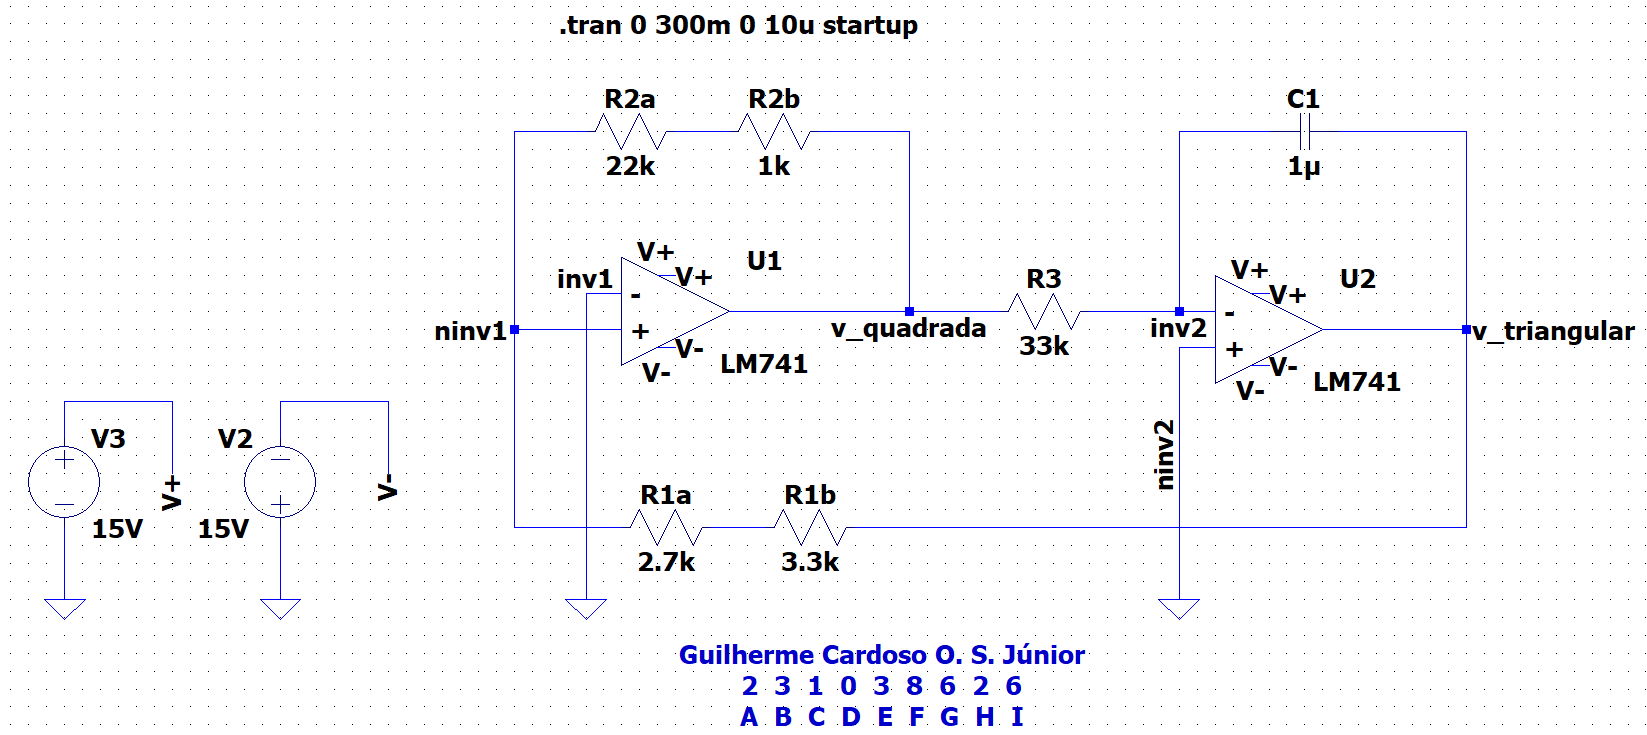
\includegraphics[width=\linewidth]{imgs/cardoso/esquematicos/item_2_esquemático.png}
    \vspace{2pt}
    {\small (b) Gerador astável de onda quadrada e triangular em malha fechada.}
\end{minipage}

\vspace{12pt}

\begin{minipage}{0.96\linewidth}
    \centering
    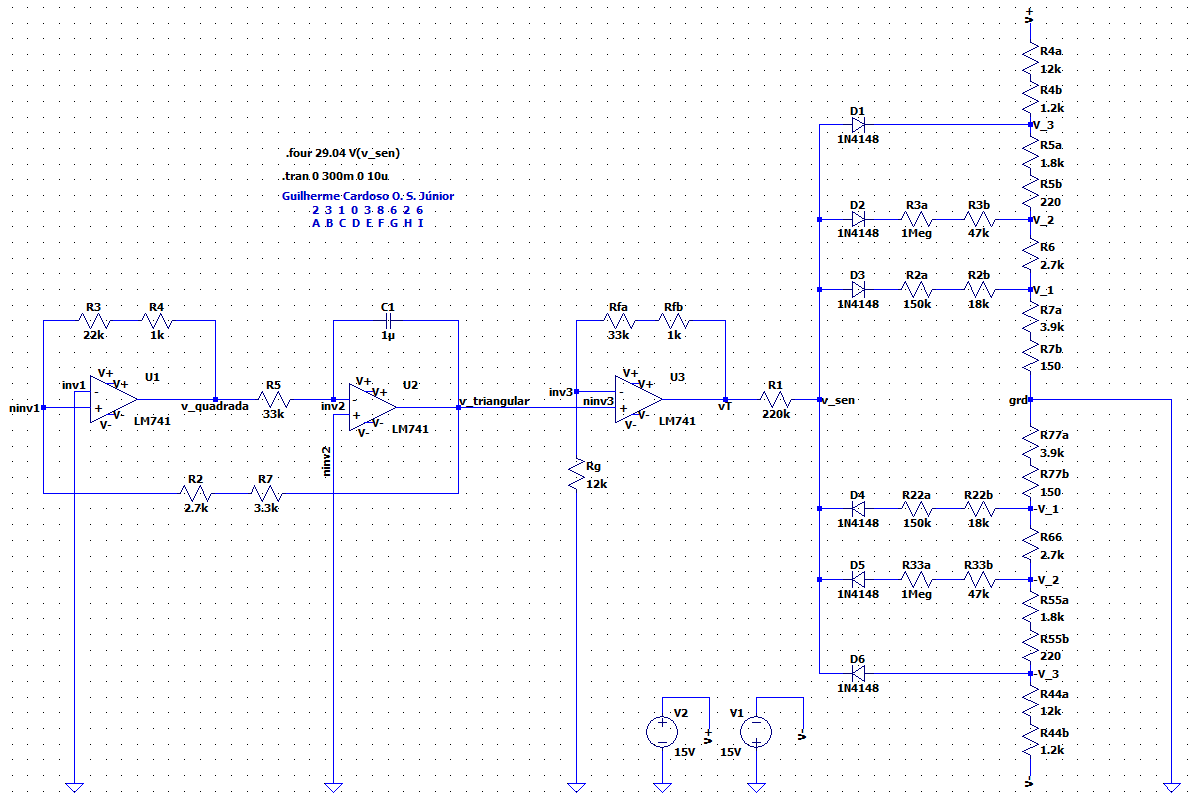
\includegraphics[width=\linewidth]{imgs/cardoso/esquematicos/item_3_esquemático.png}
    \vspace{2pt}
    {\small (c) Cadeia completa do oscilador acoplada ao estágio conformador a diodos simétrico.}
\end{minipage}

\caption{Esquemáticos projetados no LTspice para a matrícula 23/1038626, detalhando as associações da série E12 e a integração sucessiva dos estágios.}
\label{fig:circs_guilherme}
\end{figure}

% Cada integrante recebeu uma especificação diferente da própria matrícula, e portanto chegou
% a um dimensionamento diferente. Traga aqui \textbf{uma simulação por integrante}, cada uma
% com os componentes que aquela pessoa projetou. São elas que mostram se cada projeto cumpre
% o que foi pedido.

\subsection{Montagem em bancada}

% A equipe monta um circuito só. Diga \textbf{de quem} é a especificação que vocês montaram e
% por que escolheram essa. Informe os valores \textbf{medidos} de cada componente que vocês
% usaram, e não os valores nominais impressos no corpo da peça, porque a diferença entre os
% dois explica boa parte do que vocês vão observar.

\subsection{Simulação da montagem}

% Refaça a simulação usando os valores medidos dos componentes que estavam na bancada. Ela
% não substitui a simulação de projeto: é a comparação entre as duas que separa o efeito da
% tolerância dos componentes do restante.

\begin{nota}{Três comparações, três causas diferentes}
% Ao longo do relatório vocês vão confrontar três pares de resultados. Cada um responde a uma
% pergunta distinta, e vale mantê-los separados na hora de discutir.

% \smallskip
% \textbf{Cálculo analítico contra simulação de projeto.} A conta está certa? Se aqui houver
% diferença, procure na álgebra ou no esquemático.

% \smallskip
% \textbf{Simulação de projeto contra simulação da montagem.} Quanto custou a tolerância dos
% componentes? A diferença aqui é a distância entre o valor nominal e o valor real da peça
% que vocês pegaram.

% \smallskip
% \textbf{Simulação da montagem contra medição.} O modelo descreve o circuito real? Diferença
% aqui aponta algo que o modelo não representa, como a resistência série do indutor, a
% impedância da ponta de prova ou a banda do instrumento.
\end{nota}

% \begin{figure}[htb]
% \centering
% % \includegraphics[width=0.8\linewidth]{arquivo.png}
% \fbox{\parbox[c][3.2cm][c]{0.8\linewidth}{\centering\color{cinza}
%   substitua por \texttt{\textbackslash includegraphics}}}
% \caption{Legenda descritiva. Diga o que a figura mostra e o que nela é relevante, e não
% apenas o nome do circuito.}
% \label{fig:exemplo}
% \end{figure}

\section{Resultados}

% Apresente o que vocês obtiveram, em tabela sempre que houver mais de dois números. Use o
% número de algarismos significativos que a medição sustenta, e não todos os que o programa
% imprime. Para cada leitura de bancada, informe o instrumento e a incerteza.

% Guarde a interpretação para a seção seguinte: aqui vocês mostram o que encontraram.

\subsection{Projeto de cada integrante}

% Uma tabela por integrante, ou uma tabela única com uma coluna por integrante, confrontando
% o valor analítico e o simulado para cada grandeza pedida no roteiro.

\section{Resultados}

% Apresente o que vocês obtiveram, em tabela sempre que houver mais de dois números. Use o
% número de algarismos significativos que a medição sustenta, e não todos os que o programa
% imprime. Para cada leitura de bancada, informe o instrumento e a incerteza.

% Guarde a interpretação para a seção seguinte: aqui vocês mostram o que encontraram.

\subsection{Projeto de cada integrante}

% Uma tabela por integrante, ou uma tabela única com uma coluna por integrante, confrontando
% o valor analítico e o simulado para cada grandeza pedida no roteiro.

\subsubsection{Guilherme Cardoso Oliveira da Silva Júnior (23/1038626)}

A Tabela~\ref{tab:resultados_cardoso} apresenta os parâmetros projetados analiticamente a partir dos componentes da série E12, confrontando-os com os resultados medidos nas simulações de regime transitório (\texttt{.tran}) no LTspice, extraídos via diretivas \texttt{.meas}.

\begin{table}[H]
    \centering
    \caption{Resultados simulados dos estágios do oscilador astável e conformador (Matrícula 23/1038626).}
    \label{tab:resultados_cardoso}
    \renewcommand{\arraystretch}{1.2}
    \begin{tabular}{@{}lrrr@{}}
    \toprule
    \textbf{Grandeza} & \textbf{Analítico} & \textbf{Simulado} & \textbf{Erro (\%)} \\
    \midrule    
    Tensão de Saturação (Item 1, $V_{sat}$) & $14{,}00\text{ V}$ & $14{,}00\text{ V}$ & $0{,}00\%$ \\
    Limiar de Comutação ($+V_L$) & $3{,}65\text{ V}$ & $3{,}65\text{ V}$ & $0{,}00\%$ \\
    Frequência do Astável ($f$) & $29{,}04\text{ Hz}$ & $29{,}06\text{ Hz}$ & $0{,}07\%$ \\
    Amplitude da Onda Triangular ($V_{tri}$) & $3{,}65\text{ V}$ & $3{,}62\text{ V}$ & $-0{,}82\%$ \\
    Pico da Saída do Amplificador ($V_T$) & $14{,}00\text{ V}$ & $13{,}90\text{ V}$ & $-0{,}71\%$ \\
    Amplitude da Pseudossenoide ($A$) & $7{,}00\text{ V}$ & $6{,}50\text{ V}$ & $-7{,}14\%$ \\
    Distorção Harmônica Total (THD) & $\le 10\%$ & $6{,}54\%$ & -- \\
    \bottomrule
    \end{tabular}
\end{table}

\paragraph{Análise do Comparador com Histerese (Item 1):}
Alimentado por tensões simétricas de $\pm15\text{ V}$, o amplificador LM741 operou na saturação, entregando cravados $\pm14{,}00\text{ V}$ na saída. A simulação confirmou perfeitamente o cálculo teórico dos limiares de histerese (Eq. 1): comutando sempre que o sinal de excitação senoidal cruzava $\pm 3{,}65\text{ V}$, o que comprova que o divisor resistivo na malha de realimentação positiva ($R_1 = 6\text{ k}\Omega$ e $R_2 = 23\text{ k}\Omega$) fixa adequadamente as tensões de instabilidade.

\paragraph{Análise do Gerador de Ondas (Item 2):}
Fechando a malha com o estágio integrador, a dinâmica de oscilação ocorreu livremente a partir da partida (\texttt{startup}). A simulação mediu uma frequência de $29{,}06\text{ Hz}$, desvio irrelevante (inferior a $0{,}1\%$) em relação à previsão analítica (Eq. 3). A amplitude de pico da onda triangular alcançou $3{,}62\text{ V}$, também alinhada à expectativa teórica limitadora imposta pelos limiares do próprio comparador (Eq. 2). A onda quadrada gerada cravou aproximadamente $\pm13{,}96\text{ V}$, limitando levemente o $V_{sat}$ devido às quedas de tensão internas dos estágios acoplados.

\paragraph{Análise do Conformador e THD (Item 3):}
Na cadeia completa, o amplificador não inversor resgatou a tensão do sinal triangular, elevando o pico de saída ($V_T$) para $13{,}90\text{ V}$, virtualmente próximo aos $14\text{ V}$ desejados. 
Após atravessar as três malhas do conformador não linear simétrico, o sinal atingiu um pico pseudossenoidal ($V_{sen}$) de $6{,}50\text{ V}$. O erro de cerca de $-7\%$ frente à amplitude alvo ($7\text{ V}$) justifica-se pelas aproximações compulsórias dos valores resistivos impostas pela série comercial E12 nos nós de inclinação (principalmente em $R_3$). O LTspice realizou a análise de Fourier do sinal gerado (diretiva \texttt{.four}) e acusou uma Distorção Harmônica Total (THD) de apenas $6{,}54\%$. Essa distorção é considerada um excelente resultado de suavização, dado que a topologia implementa apenas três quebras resistivas e alcançou uma qualidade espectral que atende tipicamente aos padrões gerais de geradores de laboratório didático.

\begin{figure}[H]
    \centering
    \begin{minipage}[b]{0.48\linewidth}
        \centering
        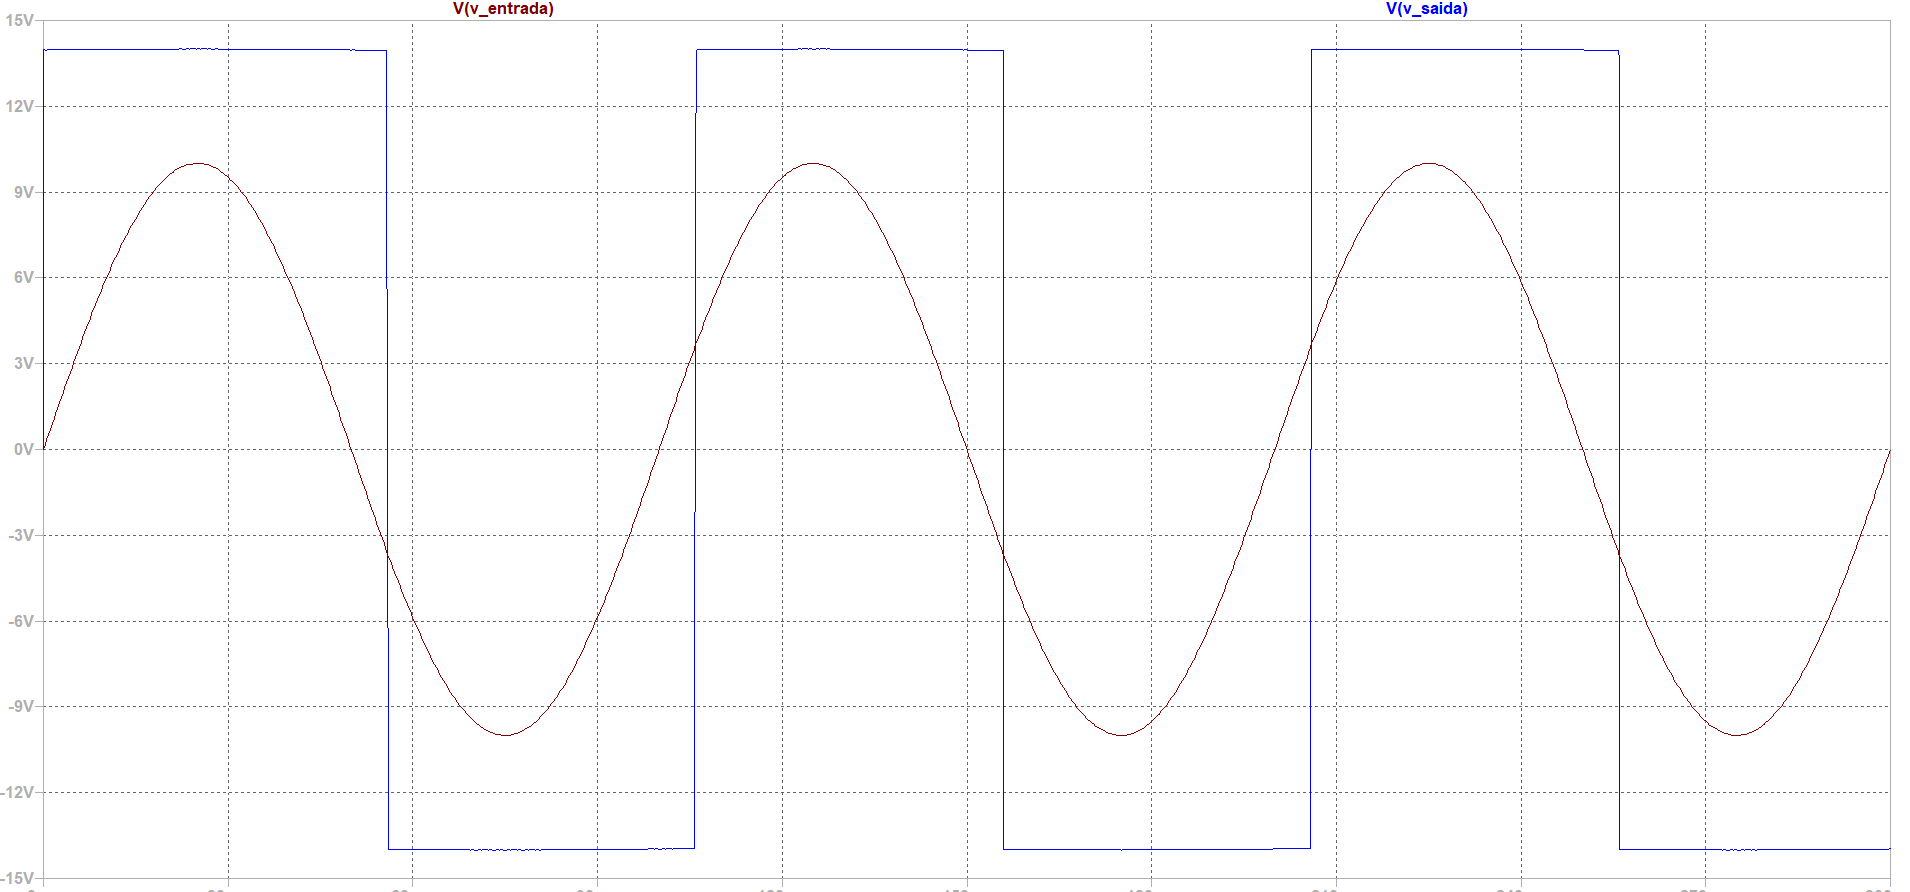
\includegraphics[width=\linewidth]{imgs/cardoso/resultados/simulacao_item_1_exp6.png}
        \vspace{2pt}
        {\small (a) Tensão: Comparador com histerese no domínio do tempo.}
    \end{minipage}%
    \hfill
    \begin{minipage}[b]{0.48\linewidth}
        \centering
        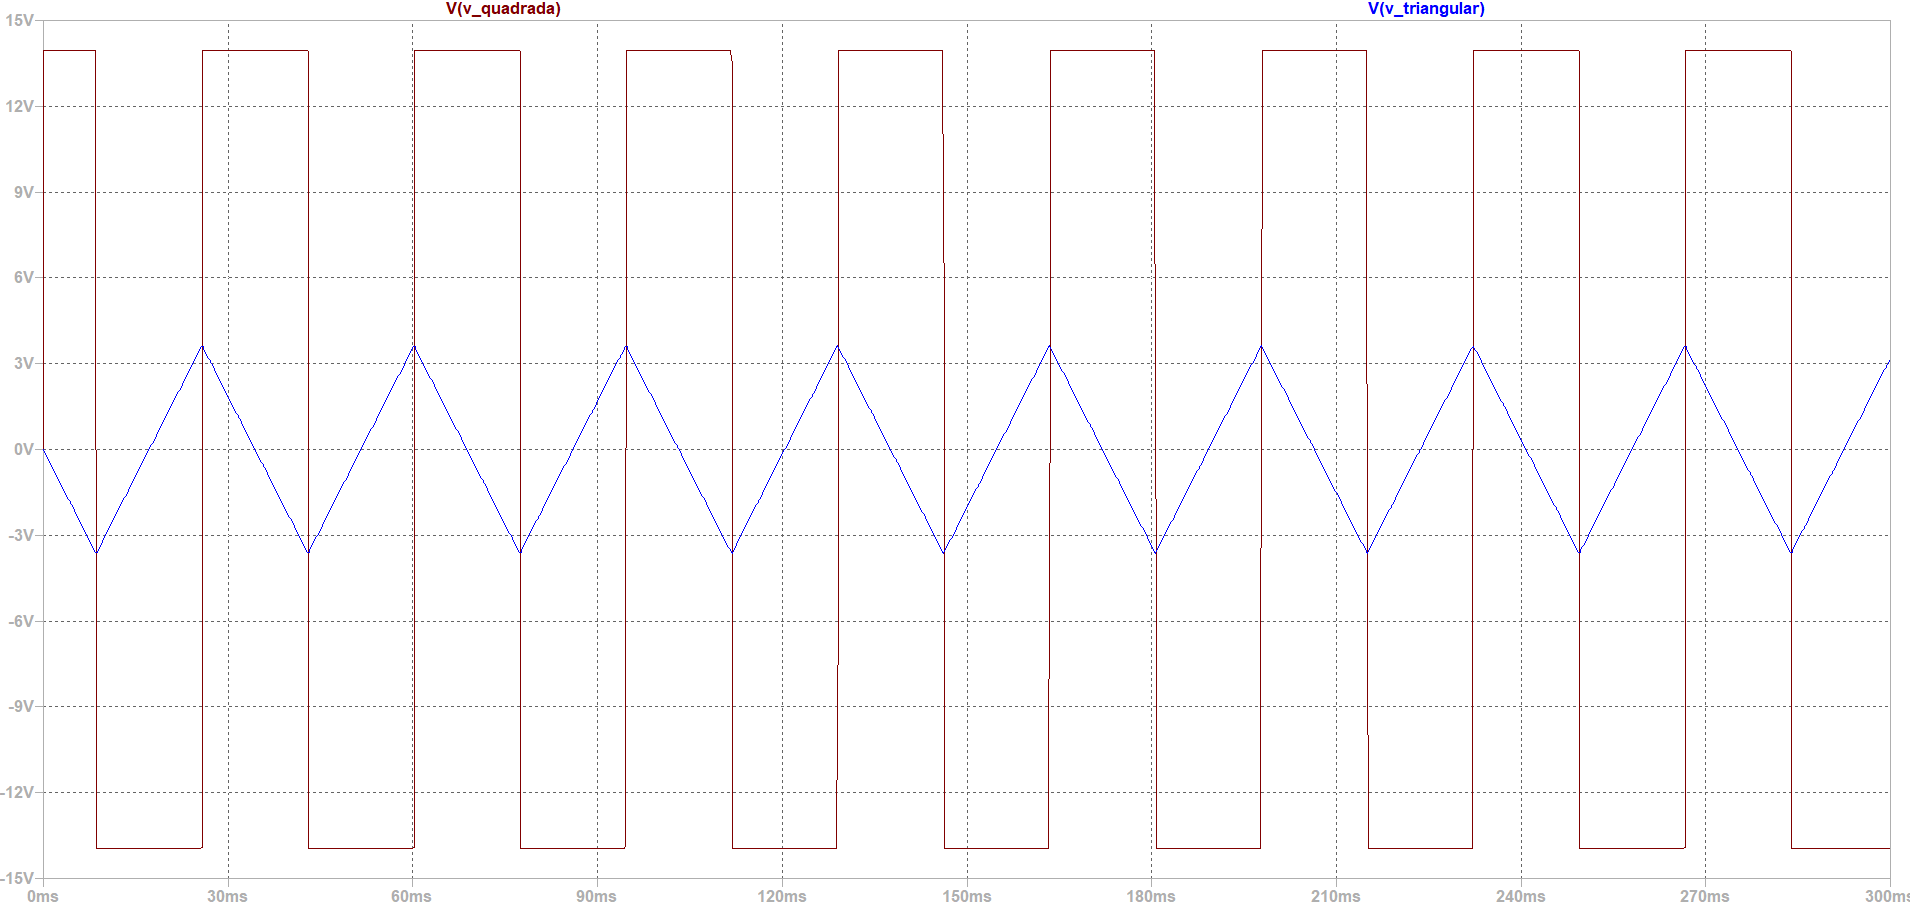
\includegraphics[width=\linewidth]{imgs/cardoso/resultados/simulacao_item_2_exp6.png}
        \vspace{2pt}
        {\small (b) Tensão: Gerador Astável (Onda Quadrada e Triangular).}
    \end{minipage}

    \vspace{12pt}

    \begin{minipage}[b]{0.48\linewidth}
        \centering
        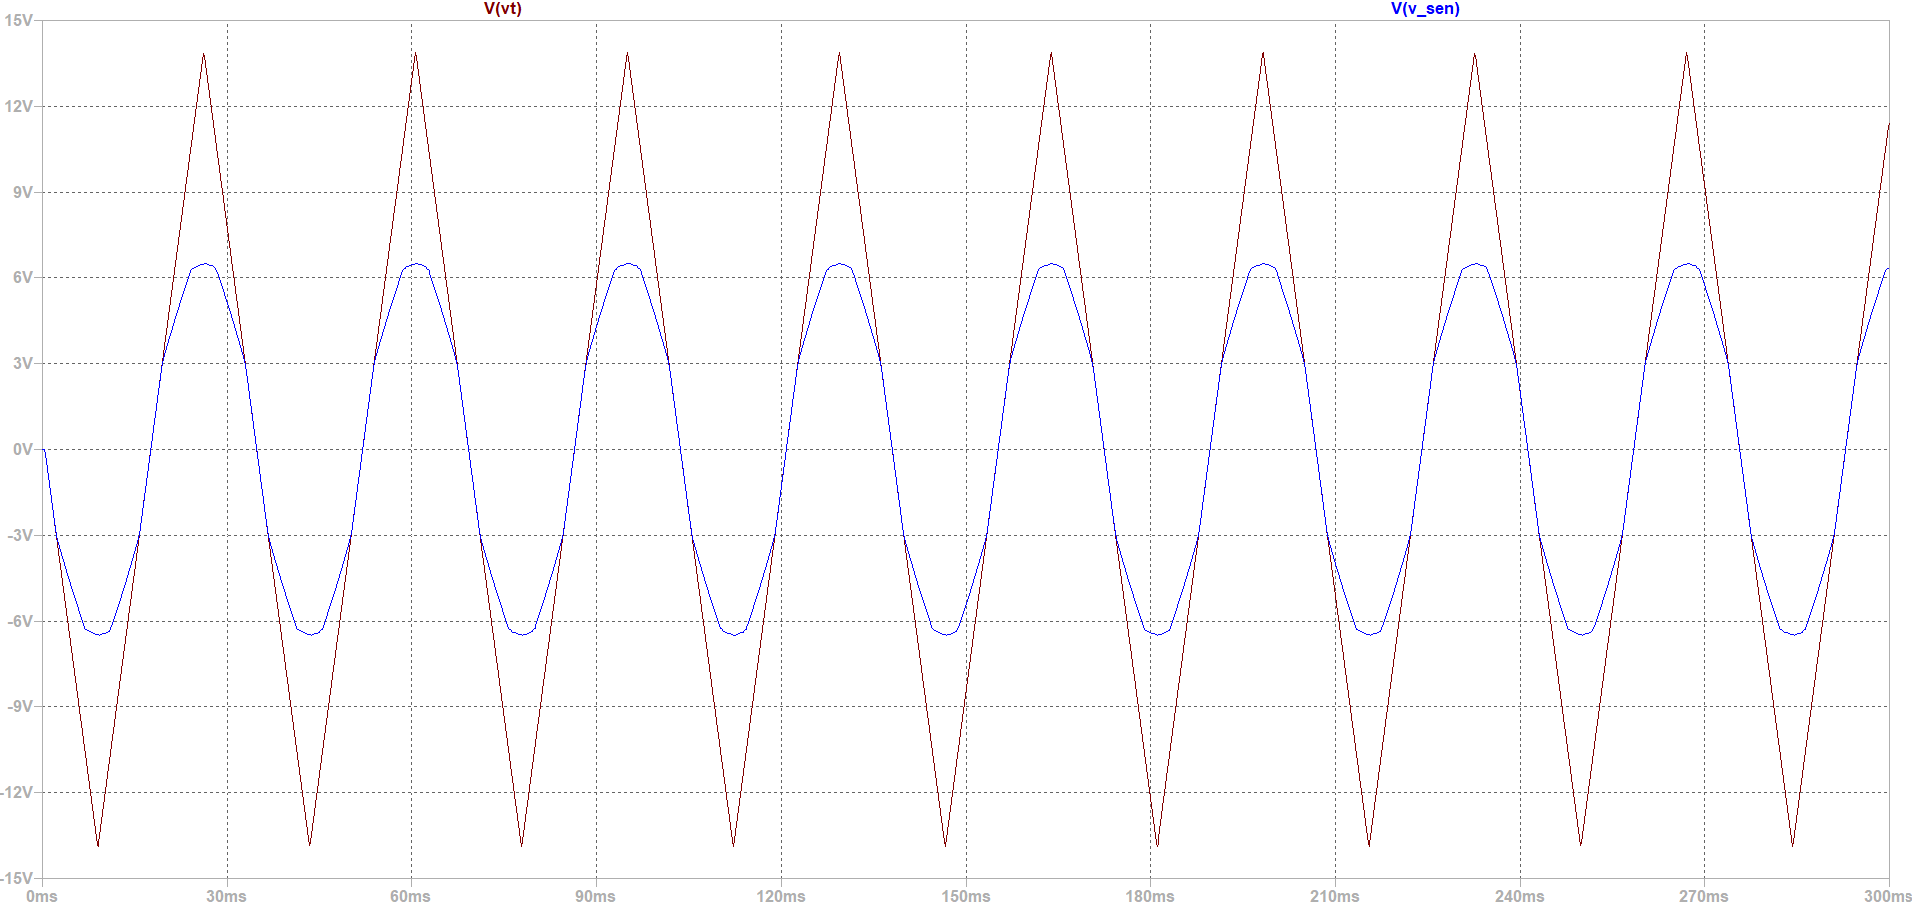
\includegraphics[width=\linewidth]{imgs/cardoso/resultados/simulacao_item_3_tempo.png}
        \vspace{2pt}
        {\small (c) Tensão: Triângulo de entrada e Pseudossenoide final.}
    \end{minipage}
    \hfill
    \begin{minipage}[b]{0.48\linewidth}
        \centering
        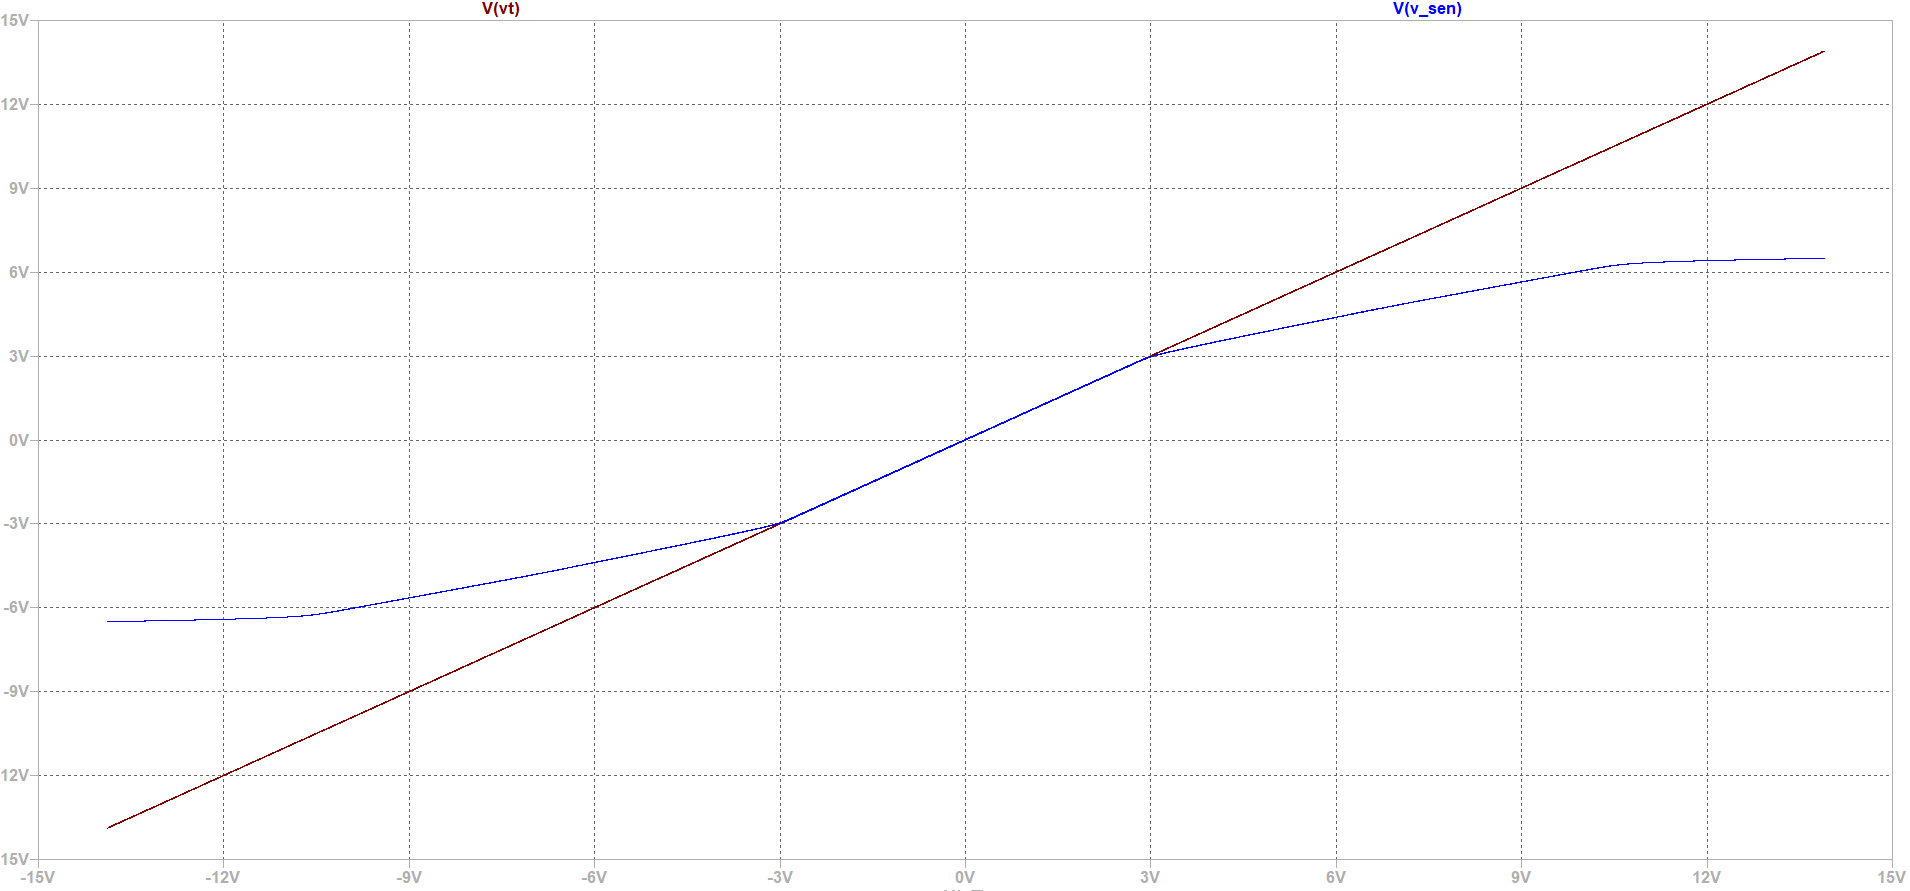
\includegraphics[width=\linewidth]{imgs/cardoso/resultados/simulacao_item_3_xy.png}
        \vspace{2pt}
        {\small (d) Curva XY: Função de transferência do conformador e quebras de ganho.}
    \end{minipage}
    \caption{Resultados gráficos das simulações dos estágios do Roteiro 6.}
    \label{fig:graficos_cardoso}
\end{figure}

\subsection{Circuito montado}

% Para cada grandeza, o que o projeto do integrante montado previa, o que a simulação com os
% valores medidos devolveu, e o que vocês mediram na bancada. É desta tabela que sai a
% discussão.

% \begin{center}
% \begin{tabular}{@{}lrrrr@{}}
% \toprule
% \textbf{Grandeza} & \textbf{Projeto} & \textbf{Sim. montagem} & \textbf{Medido} &
% \textbf{Erro} \\
% \midrule
% & & & & \\
% \bottomrule
% \end{tabular}
% \end{center}

\section{Discussão}

% Percorra as três comparações na ordem em que aparecem no quadro da Seção~4: a conta contra
% a simulação de projeto, esta contra a simulação da montagem, e esta contra a medição. Cada
% passo isola uma causa, e a discussão fica bem mais curta quando eles não se misturam.

% Compare também os projetos dos integrantes entre si. Como as especificações são diferentes,
% os resultados diferem, e mostrar que essa diferença é a que a teoria previa vale mais do
% que repetir três vezes a mesma análise.

% Sempre que uma divergência for maior do que a incerteza esperada, aponte uma causa concreta
% e diga como ela poderia ser reduzida. Vale, por exemplo, a tolerância do componente, a
% resistência série do indutor, a impedância de entrada do osciloscópio, a banda do
% amplificador ou a resolução da varredura.

% Quando previsto e obtido coincidirem, explique por que era esperado que coincidissem, e o
% que essa coincidência não permite concluir.

% Por fim, retome as hipóteses que vocês declararam na fundamentação e diga quais se
% confirmaram. Se algo observado contrariar a previsão, resolva a contradição aqui.

\section{Conclusão}

% Retome o objetivo que vocês anunciaram na introdução e responda se ele foi atingido,
% apoiando a resposta em um número. Aponte a principal limitação do que foi feito e o que
% ela impede de afirmar. Evite trazer resultado novo nesta seção.

\section{Referências}

\begin{referencias}
\item SEDRA, A.~S.; SMITH, K.~C. \emph{Microeletrônica}. 5.~ed. São Paulo: Pearson
      Prentice Hall, 2007.
\item BOYLESTAD, R.~L.; NASHELSKY, L. \emph{Dispositivos Eletrônicos e Teoria de
      Circuitos}. 11.~ed. São Paulo: Pearson Education do Brasil, 2013.
\end{referencias}

\end{document}
